%%%%%%%%%%%%%%%%%%%%%%%%%%%%%%%%%%%%%%%%%%%%%%%%%%%%%%%%%%%%%%%%%%%%%%%%
%                                                                      %
%     File: Thesis_Appendix_C.tex                                      %
%     Tex Master: Thesis.tex                                           %
%                                                                      %
%     Author: Israel Sother                                            %
%     Last modified: 27 May 2024                                       %
%                                                                      %
%%%%%%%%%%%%%%%%%%%%%%%%%%%%%%%%%%%%%%%%%%%%%%%%%%%%%%%%%%%%%%%%%%%%%%%%
\chapter{Current Reference using characterized inductances}
\label{chapter:appendix_current_reference}

As explained in \Cref{section:inductance_curves_current_reference}, the used current references on the experimental results were not calculated using the inductance values obtained from the motor characterization. This section presents the current references calculated using the characterized curves.

\begin{figure}[!htb]
	\begin{subfigmatrix}{2}
		\subfigure[Minimum Voltage]{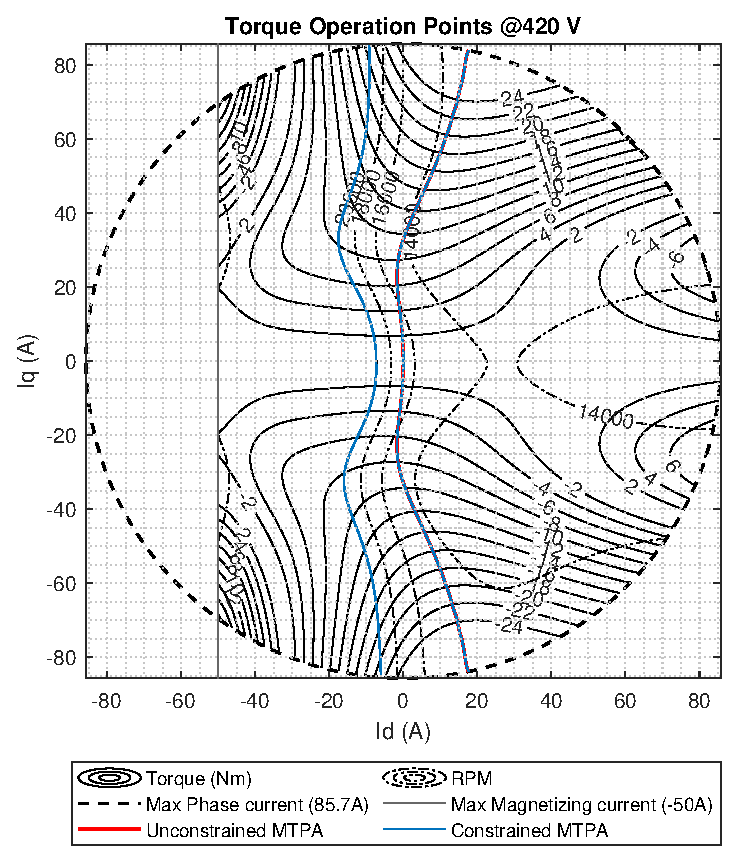
\includegraphics[width=0.49\linewidth]{Figures/Motor_map@420V_charact}\label{fig:mtpa_Constrained_420_charac}}
		\subfigure[Nominal Voltage]{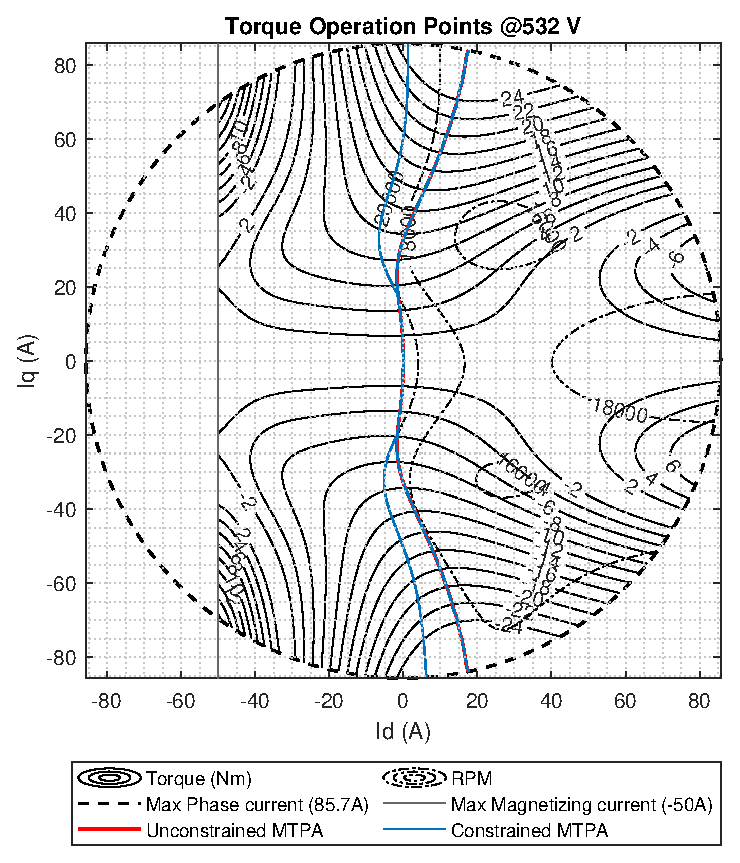
\includegraphics[width=0.49\linewidth]{Figures/Motor_map@532V_charact}\label{fig:mtpa_Constrained_540_charac}}
	\end{subfigmatrix}
	\begin{subfigmatrix}{1}
		\subfigure[Maximum Voltage]{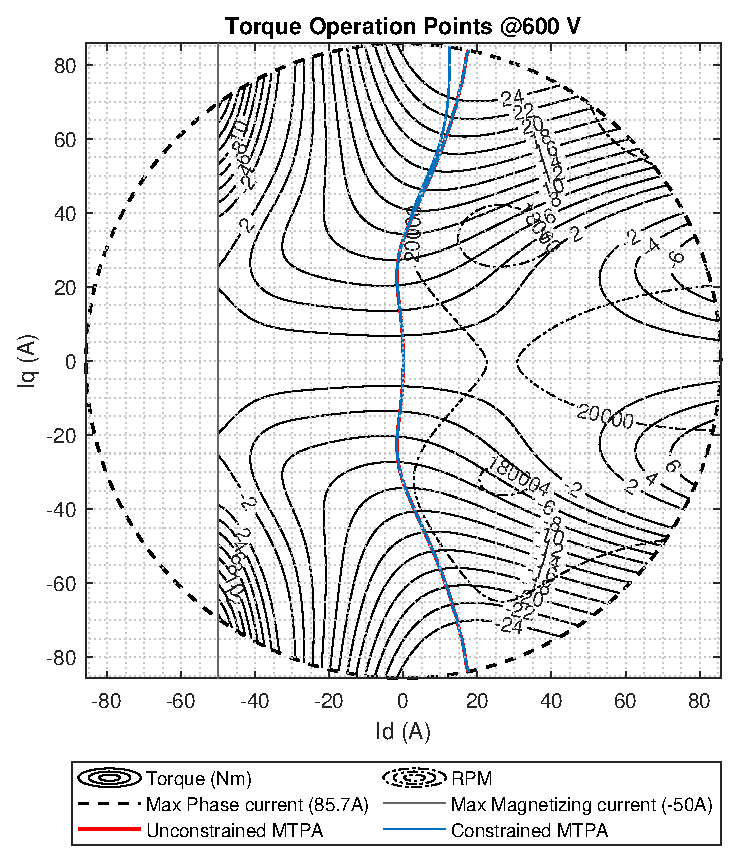
\includegraphics[width=0.49\linewidth]{Figures/Motor_map@600V_charact}\label{fig:mtpa_Constrained_588_charac}}
	\end{subfigmatrix}
	\caption{Constrained Maximum Torque per Ampere curve at minimum, nominal, and maximum voltages. Reference currents are shown for 0, 13000 and 2000 RPMs.}
	\label{fig:mtpa_constrained_new}%chktex 24
\end{figure}

An important distinction to make is that the curves in \Cref{fig:mtpa_constrained_new} present an inversion in torque signal depending on the direct axis current. This is due to the reluctance torque reaching and surpassing the torque generated by the permanent magnets. This phenomenon is due to the saturation effect, which reduces the quadrature axis inductance, while the direct axis inductance increases.